% <- percent signs are used to comment
\documentclass[12pt]{article}

%%%%%% PACKAGES - this part loads additional material for LaTeX %%%%%%%%%
% Nearly anything you want can be done in LaTeX if you load the right package 
% (search ctan.org or google it if you are looking for something).  We will load
% here a few that we need for this document or that we expect you to need later.

% The next 3 lines are needed to fix shortcomings of TeX that only make sense given its 40-year history ...
% Simple keep and ignore.
\usepackage[utf8]{inputenc}
\usepackage[T1]{fontenc}
\usepackage{lmodern}


% Custom margins (and paper sizes etc.) because LaTeX else wastes much space
\usepackage[margin=1in]{geometry}

% The following packages are created by the American Mathematical Society (AMS)
% and provide lots of tools for special fonts, symbols, theorems, and proof
\usepackage{amsmath,amsfonts,amssymb,amsthm}
% mathtools contains many detail improvements over ams and core tex
\usepackage{mathtools}

% graphicx is required for images
\usepackage{graphicx}

% enumitem used for customizing enumerations
\usepackage[shortlabels]{enumitem}

% tikz is the package used for drawing, in particular for drawing trees. You may also find simplified packages like tikz-qtree and forest useful
\usepackage{tikz}

% hyperref allows links, urls, and many other PDF tricks.  We load it here
%          in such a way that the PDF file has info about it
\usepackage[%
	pdftitle={CS240 Assignment 0},%
	hidelinks,%
]{hyperref}


%%%%%% COMMANDS - here you can define your own LaTeX-commands %%%%%%%%%

%%%%%% End of Preamble %%%%%%%%%%%%%

\begin{document}

\begin{center}
{\Large\textbf{OMERS "SMASHERS" Work Chat}}\\
\vspace{3mm}
{\Large\textbf{Fall 2022}}\\
\vspace{2mm}
{\Large\textbf{Unmuting Factum}}\\
\vspace{3mm}
\textbf{Due Date: Monday, October 17th, 2022 at 11:32am}
\end{center}

\section*{Background}

On the date of October 17th, 2022 at 11:13am EST a shocking revelation was made; Gina a dear member of "SMASHERS"
\footnote{%
	An entirely OMERS sanctioned business group which meets often about NFTs, and other Smash NFRS%
} 
muted the chat, much to the sheer anguish of Jonathan and myself.

% An empty line starts a new paragraph.

As such this document seeks to prove the mathematical validity of keeping the chat unmuted, without loss of generality each proof with defiantly make the case of staying in the chat.
\vspace{15mm}
\begin{center}
(Also I wanna point out how much of a pain it is to write in latex SMH)
\end{center}

% Clearpage starts a new page, unless (by chance) a page break happens to be here anyway
\clearpage

\addtocounter{section}{-1}
% We can move number of any counter up or down.  Normally it starts at 1; here we start at 0.
\section{Academic Integrity Declaration}

I declare the following statements to be true, effective from the release of 
the aforementioned assessment until its due date and time: 
\begin{itemize}
\item The work I submit here is entirely my own. 
\item I will not use/have not used any unauthorized aids to complete this assessment. 
Unauthorized aids include but are not limited to
     - the Internet
     - someone else's solutions or partial solutions
NOTE:  if you are unsure if something is unauthorized, check with course staff 
before using it. 
\item Because this is an assignment, I may discuss it with others but will not write, 
type, take pictures, or by any other means capture what occurred during the meeting 
and will/did wait at least 30 minutes before recording anything from that meeting. 
\item I have not and will not share in whole or in part email/files/documents related 
to the solutions of the assessment except possibly with course staff. 
\item I am aware that misconduct related to assessments can result in significant 
penalties, including, zero on the assessment, overall grade deduction and, depending 
on the significance of the assessment, failing the course and suspension (this is 
covered in Policy 71: 
https://uwaterloo.ca/secretariat/policies-procedures-guidelines/policy-71). 

\end{itemize}
--> Student Quest username: r2knowle


\section{Happiness Contrapositive}
% We can assign a label to each section (and also many other things, such as 
% figures, lemmas, ...) and then refer to them.  For this to be correct, the
% file must be translated twice.
\label{sec:assignment-guidelines}

Currently, the premise that "muting the smash chat" can be described as the following first order logic function:
\[ \sum = \{\forall{x},\forall{y}(\neg G(x) \land \neg N(y) \implies \text{should mute} \} \]
Where $G(x)$ represents all instances where you are having fun, and $N(y)$ represents all the instances where you learn more about super secret guy lore. Moreover we can reduce this equation via contrapositive:
\[ \sum = \{\exists{x},\exists{y}(G(x) \lor N(y) \implies \text{should not mute} \} \]
Therefore since we know G(x) has been satisfied at least once, as you did have fun when Jonathan showed his lego batman mask, this logically and syntactical proves you should stay unmuted!

\section{Halting Problem Proof}

To prove this, we shall reduce this to the halting problem.
Assume for the sake of contradiction that this problem is decidable; therefore, a decider (D) exists such that it takes in a machine and outputs if it accepts Gina muting the chat. This machine will look like:

If the machine does accept a finite language, it outputs yes and halts otherwise it outputs no and loops. Let’s say that we have some candidates (M,w) for the halting problem, where w is some finite language.  We can construct a new algorithm to decide the halting of M on w where CONVERT is a turning machine that takes M and w in as inputs and creates a machine ($M_w$) that is passed to the decider defined above:

\begin{figure}[tbhp]
	\begin{center}
		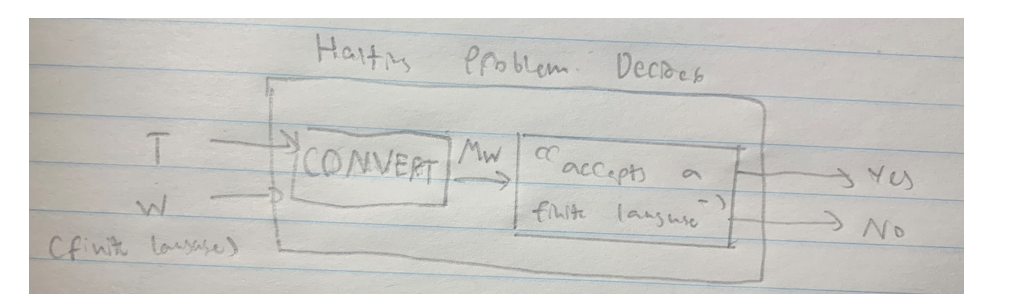
\includegraphics[width=0.7\textwidth]{p2.png}
	\end{center}
\end{figure}

This turning machine will halt on input w if $M_w$ halts on the input of an infinite language. Thus because we have built a decider for the halting problem, this problem cant be decidable and thus Gina should keep that chat unmuted.

\section{Pathos Appeal}
\label{sec:image}

Look at this silly goofy guy:

\begin{figure}[tbhp]
	\begin{center}
		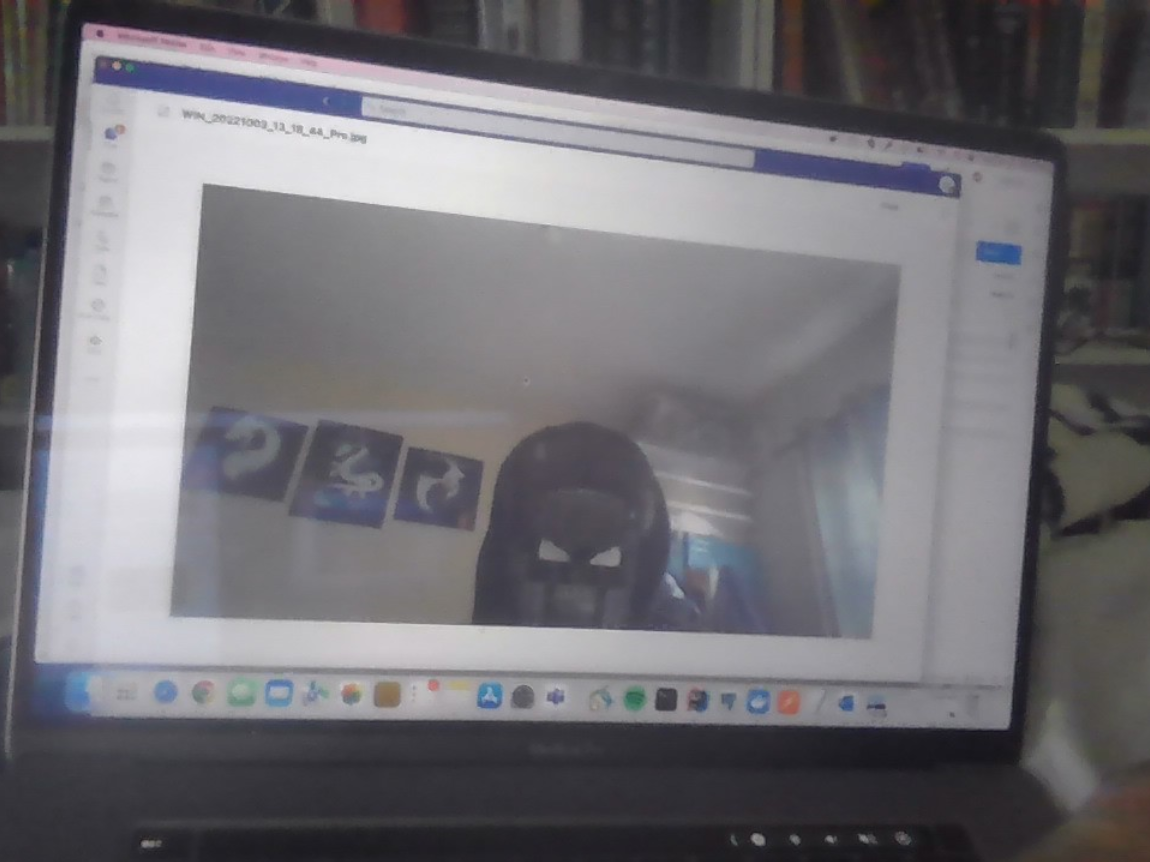
\includegraphics[width=0.5\textwidth]{p3.png}
	\end{center}
	\caption{goofy fella.}
	\label{figcaption}
\end{figure}

{\itshape Hint: he will be sad}

\end{document}